\section{Implementation on Software-defined radio}
\label{sec:real_implementation}

\begin{figure*}[t]
  \centerline{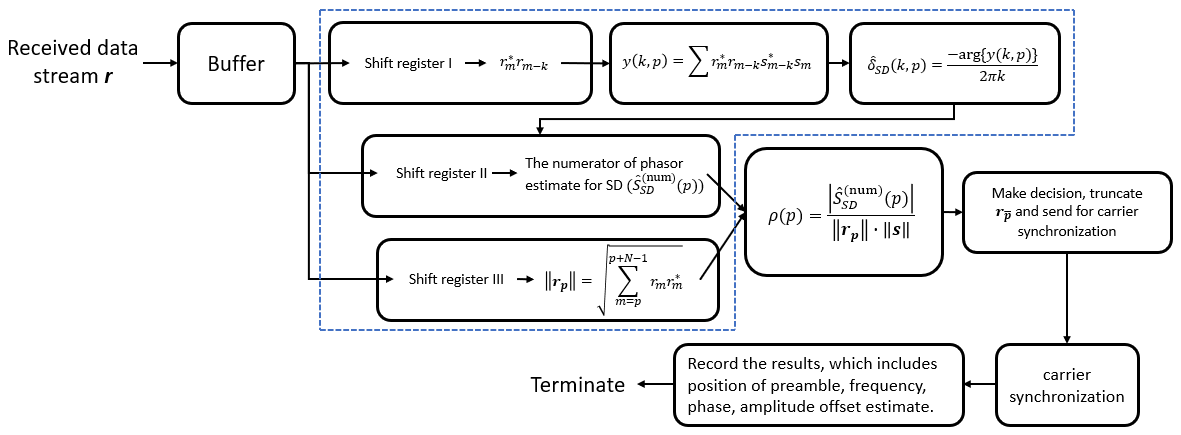
\includegraphics[width=6.5in]{SDR_receiver.png}}
  \caption{Block diagram for implementing the proposed algorithm on software-defined radio (some steps are omitted)}
  \label{fig:SDR_receiver}
  \end{figure*}

Two main aspects of measuring the performance of modern communcation systems, except for accuracy,
are the latency and throughput. In the previous sections, we focus on explaining and showing
how much accuracy of our proposed joint detection and estimation algorithm can be.
In order to realize it on software-defined radio (SDR), the algorithm, especially the detection algorithm, should be refined
to fitting very high sample rate since it is applied on every time instant.

\subsection{Receiver Side (algorithm)}

Figure~\ref{fig:SDR_receiver} illustrates some detailed changes of our proposed algorithm.
First, the style of the observation window with feedback loop in Figure~\ref{fig:sig_acquis_chain} is eliminated
because it incurs a very large amount of overhead. Instead, the received data is directly buffered into 
a fixed size (normally larger than the length of the preamble) of frame without overlapping. Now
the problem may happen when the preamble in the received data is cut off over two frames. 
The shift register is reused after the buffer to solve this problem. Compared with the old method, the received data packed in frames can be processed in order without
waiting for the result of detecting; Moreover, the length of the shift register can be also reduced. 
For example, if we look at formula of the SD estimator in~\eqref{eq:delta_SD}, the length of the shift register can be shortened from $N$ to $k+1$,
i.e., if $k=\frac{2}{3}N$, the overhead is approximately reduced by $\frac{N}{3}$.

Second, some key steps of the proposed detection algorithm should be computed more efficiently.
For example, to calculate the frequency estimate of SD estimator,~\eqref{eq:delta_SD} can be intepreted as the convolution between autocorrelation vector of received samples and of the preamble (one of them should be reversed). 
Thus, the most efficient way of calculating~\eqref{eq:delta_SD} could be the fast fourier transform (FFT). 

Another important improvement that should be emphasized is about calculating the phase (phasor) estimate
of the SD estimator in~\eqref{eq:opt_S}. No
te,~\eqref{eq:opt_S} is a time-varying convolution, which cannot be computed by FFT.
To approximate the dot product in~\eqref{eq:opt_S}, we re-order the computation by first calculating the dot product between the (partial) received data vector ($\bm{r}$) and the (partial) preamble ($\bm{s}$);
the result is then corrected (multiplied) by the frequency estimate at the middle position of data vector and added together. Specifically, the numerator of

\begin{equation}
    \label{eq:refined_opt_S}
    \hat{S} \approx \sum_{i=0}^{L_2-1} \sum_{m=iL_1/L_2}^{(i+1)L_1/L_2-1}
    \sum_{n=mN/L_1}^{(m+1)N/L_1-1}r_ns_n^* 
    e^{-j\pi \hat{\delta}\frac{N(2m+1)}{L_1}}.
  \end{equation}
As illustrated in Figure~\ref{fig:SDR_receiver}, we compute~\eqref{eq:refined_opt_S} in two stages, each
stage contains $L_1$ (or $L_2$) parallel sub cells. 
Thus, we achieve the functional parallelism by an approximate of $L_1 \cdot L_2$ speed up.
To get a good approximation, $L_1$ should not be too small and 
$L_2$ is the factor of $L_1$.

\subsection{Signal Transmission Path}

In this section, we briefly talk about the signal transmitting path, which is used 
for testing our algorithm. The hardware connection is fairly easy. 
Each of two processors (computers) connected to a universal software radio peripheral (USRP) 
by one 5-Gigabit Ethernet cable as the transmitter or receiver. Between two USRPs,
a cable with~\numb{30}\dB~attenuation connects the RX/TX port and RX port.
At the transmitter side, the processor needs to tell the (transmitter) USRP the sample rate, 
the baseband signal and frequency, the carrier frequency, the transmitter gain, etc. 
Then, the USRP transmits the analog signal to the (receiver) USRP through the two ports.
At the receiver side, the received analog RF signal is first down-converted to baseband, down-sampled to 
discrete-time data stream and finally stored in the local network. After that, our proposed algorithm as illustrated
in Figure~\ref{fig:SDR_receiver} can be tested by requesting the data from the local network.

\subsection{Performance of SDR}

To measure the performance of the SDR, we focus on the accuracy, throughput and latency of our proposed algorithm.
Some parameters in Figure~\ref{fig:SDR_receiver} should be chosen by the following rules:
First, the length of the preamble should be chosen short enough to get the largest throughput as long as it does not degrade the accuracy;
Second, the length of frame should be chosen as the power of 2 to achieve the best performance of FFT; Moreover, 
it trades off between the overhead and latency, e.g., short frame has small latency but large overhead. 
Third, as discussed above, $L_1$ in~\eqref{eq:refined_opt_S} should not be chosen too small for a good approximation of phasor estimate. However, the large number of 
parallel executions will occupy the most threads of the computer.

As tested, such parameters are determined that can achieve a relatively good performance: 
The preamble is chosen with the number of symbols $L_0=32$ and oversampling factor $M=4$.
the length of the frame is determined by 8192; Four complete preambles are embedded in each frame. 
The number of sub cells for two stages are $L_1=2L_2=16$. Furthermore, some parameters of USRP are set as follows:
The sample rate at transmitter is 10 MS/s; The transmitter gain plus receiver gain is~\numb{20}\dB.
Based on above, we get the maximum throughput is around 4.5 MS/s and the latency is near 1 ms;
The detection algorithm is very robust and the false alarm probability is near 0.


